% !Mode:: "TeX:UTF-8"
% !TEX program = xelatex

%%%%%%%%%% Port for macOS %%%%%%%%%%%
% Modified: Qin Yubo

\def\usewhat{xelatex}
\documentclass[12pt,openany,twoside]{book}
% 如果你认为文中中文逗号样式过于难看,可在Overleaf中尝试以下命令
% \documentclass[12pt,openany,twoside,fontset=ubuntu]{book}
% 也可以在windows环境下尝试以下命令,但在windows下可能会引发加粗命令失效
% \documentclass[12pt,openany,twoside,fontset=windows]{book}



%强制目录页的第一页的页眉页脚样式
\AtBeginDocument{\addtocontents{toc}{\protect\thispagestyle{only_foot}}}
                                                     % 本科生毕业论文通常采用单页排版
% !Mode:: "TeX:UTF-8"
%  Authors: 张井   Jing Zhang: prayever@gmail.com     天津大学2010级管理与经济学部信息管理与信息系统专业硕士生
%           余蓝涛 Lantao Yu: lantaoyu1991@gmail.com  天津大学2008级精密仪器与光电子工程学院测控技术与仪器专业本科生

%%%%%%%%%% Package %%%%%%%%%%%%
% \usepackage{CJK}
\usepackage{lmodern}
\usepackage[T1]{fontenc}
\usepackage{graphicx}                       % 支持插图处理
\usepackage[a4paper,text={146.4true mm,239.2 true mm},top= 26.2true mm,left=31.8 true mm,head=6true mm,headsep=6.5true mm,foot=16.5true mm]{geometry}
                                            % 支持版面尺寸设置
\usepackage[squaren]{SIunits}               % 支持国际标准单位

\usepackage{titlesec}                       % 控制标题的宏包
\usepackage{titletoc}                       % 控制目录的宏包
\usepackage{fancyhdr}                       % fancyhdr宏包 支持页眉和页脚的相关定义
\usepackage[UTF8]{ctex}                           % 支持中文显示
% \usepackage{CJKpunct}                       % 精细调整中文的标点符号
% \usepackage{color}                          % 支持彩色
\usepackage{amsmath}                        % AMSLaTeX宏包 用来排出更加漂亮的公式
\usepackage{amssymb}                        % 数学符号生成命令
\usepackage[below]{placeins}    %允许上一个section的浮动图形出现在下一个section的开始部分,还提供\FloatBarrier命令,使所有未处理的浮动图形立即被处理
\usepackage{multirow}                       % 使用Multirow宏包,使得表格可以合并多个row格
\usepackage{booktabs}                       % 表格,横的粗线;\specialrule{1pt}{0pt}{0pt}
\usepackage{longtable}                      % 支持跨页的表格。
\usepackage{tabularx}                       % 自动设置表格的列宽
\usepackage{subfigure}                      % 支持子图 %centerlast 设置最后一行是否居中
\usepackage[subfigure]{ccaption}            % 支持子图的中文标题
\usepackage[sort&compress,numbers]{natbib}  % 支持引用缩写的宏包
\usepackage{enumitem}                       % 使用enumitem宏包,改变列表项的格式
\usepackage{calc}                           % 长度可以用+ - * / 进行计算
\usepackage{txfonts}                        % 字体宏包
\usepackage{bm}                             % 处理数学公式中的黑斜体的宏包
\usepackage[amsmath,thmmarks,hyperref]{ntheorem}  % 定理类环境宏包,其中 amsmath 选项用来兼容 AMS LaTeX 的宏包

%\usepackage{CJKnumb}                        % 提供将阿拉伯数字转换成中文数字的命令
\usepackage{indentfirst}                    % 首行缩进宏包
% \usepackage{CJKutf8}                        % 用在UTF8编码环境下,它可以自动调用CJK,同时针对UTF8编码作了设置
%\usepackage{hypbmsec}                      % 用来控制书签中标题显示内容
\newcommand{\tabincell}[2]{\begin{tabular}{@{}#1@{}}#2\end{tabular}}
\usepackage{xcolor}
\usepackage{threeparttable}                 %支持对表格中的数据进行注释
%支持代码环境
\usepackage{listings}
\lstset{numbers=left,
language=[ANSI]{C},
numberstyle=\tiny,
extendedchars=false,
showstringspaces=false,
breakatwhitespace=false,
breaklines=true,
captionpos=b,
keywordstyle=\color{blue!70},
commentstyle=\color{red!50!green!50!blue!50},
frame=shadowbox,
rulesepcolor=\color{red!20!green!20!blue!20}
}
%支持算法环境
\usepackage[boxed,ruled,lined]{algorithm2e}
\usepackage{algorithmic}

\usepackage{array}
\newcommand{\PreserveBackslash}[1]{\let\temp=\\#1\let\\=\temp}
\newcolumntype{C}[1]{>{\PreserveBackslash\centering}p{#1}}
\newcolumntype{R}[1]{>{\PreserveBackslash\raggedleft}p{#1}}
\newcolumntype{L}[1]{>{\PreserveBackslash\raggedright}p{#1}}

\def\atemp{xelatex}\ifx\atemp\usewhat
\usepackage[unicode,
            pdfstartview=FitH,
            bookmarksnumbered=true,
            bookmarksopen=true,
            colorlinks=false,
            pdfborder={0 0 1},
            citecolor=blue,
            linkcolor=red,
            anchorcolor=green,
            urlcolor=blue,
            breaklinks=true
            ]{hyperref}
\fi

                                % 定义本文所使用宏包
\graphicspath{{figures/}}                            % 定义所有的图像文件在 figures 子目录下
\begin{document}                                     % 开始全文
% !Mode:: "TeX:UTF-8"
%  Authors: 张井   Jing Zhang: prayever@gmail.com     天津大学2010级管理与经济学部信息管理与信息系统专业硕士生
%           余蓝涛 Lantao Yu: lantaoyu1991@gmail.com  天津大学2008级精密仪器与光电子工程学院测控技术与仪器专业本科生

%%%%%%%%%% Fonts Definition and Basics %%%%%%%%%%%%%%%%%
\newcommand{\song}{\songti}    % 宋体
\newcommand{\fs}{\fangsong}        % 仿宋体
\newcommand{\kai}{\kaishu}      % 楷体
\newcommand{\hei}{\heiti}      % 黑体
\newcommand{\li}{\lishu}        % 隶书
\newcommand{\kaiGB}{\CJKfamily{kai}}      % 楷体GB2312, 用于独创性说明
\newcommand{\yihao}{\fontsize{26pt}{26pt}\selectfont}       % 一号, 1.倍行距
\newcommand{\xiaoyi}{\fontsize{24pt}{24pt}\selectfont}      % 小一, 1.倍行距
\newcommand{\erhao}{\fontsize{22pt}{1.25\baselineskip}\selectfont}       % 二号, 1.25倍行距
\newcommand{\xiaoer}{\fontsize{18pt}{18pt}\selectfont}      % 小二, 单倍行距
\newcommand{\sanhao}{\fontsize{16pt}{16pt}\selectfont}      % 三号, 1.倍行距
\newcommand{\xiaosan}{\fontsize{15pt}{15pt}\selectfont}     % 小三, 1.倍行距
\newcommand{\sihao}{\fontsize{14pt}{14pt}\selectfont}       % 四号, 1.0倍行距
\newcommand{\xiaosi}{\fontsize{12pt}{20pt}\selectfont}      % 小四, 1.倍行距
\newcommand{\wuhao}{\fontsize{10.5pt}{10.5pt}\selectfont}   % 五号, 单倍行距
\newcommand{\xiaowu}{\fontsize{9pt}{9pt}\selectfont}        % 小五, 单倍行距

\setmainfont{Times New Roman}

%\CJKcaption{gb_452}
%\CJKtilde  % 重新定义了波浪符~的意义
\newcommand\prechaptername{第}
\newcommand\postchaptername{章}

% 调整罗列环境的布局
\setitemize{leftmargin=3em,itemsep=0em,partopsep=0em,parsep=0em,topsep=-0em}
\setenumerate{leftmargin=3em,itemsep=0em,partopsep=0em,parsep=0em,topsep=0em}
%\setlength{\baselineskip}{20pt}
%\renewcommand{\baselinestretch}{1.38} % 设置行距

%避免宏包 hyperref 和 arydshln 不兼容带来的目录链接失效的问题。
\def\temp{\relax}
\let\temp\addcontentsline
\gdef\addcontentsline{\phantomsection\temp}

% 自定义项目列表标签及格式 \begin{publist} 列表项 \end{publist}
\newcounter{pubctr} %自定义新计数器
\newenvironment{publist}{%%%%%定义新环境
\begin{list}{[\arabic{pubctr}]} %%标签格式
    {
     \usecounter{pubctr}
     \setlength{\leftmargin}{2.5em}     % 左边界 \leftmargin =\itemindent + \labelwidth + \labelsep
     \setlength{\itemindent}{0em}     % 标号缩进量
     \setlength{\labelsep}{1em}       % 标号和列表项之间的距离,默认0.5em
     \setlength{\rightmargin}{0em}    % 右边界
     \setlength{\topsep}{0ex}         % 列表到上下文的垂直距离
     \setlength{\parsep}{0ex}         % 段落间距
     \setlength{\itemsep}{0ex}        % 标签间距
     \setlength{\listparindent}{0pt} % 段落缩进量
    }}
{\end{list}}%%%%%

\makeatletter
\renewcommand\normalsize{
  \@setfontsize\normalsize{12pt}{12pt} % 小四对应12pt
  \setlength\abovedisplayskip{4pt}
  \setlength\abovedisplayshortskip{4pt}
  \setlength\belowdisplayskip{\abovedisplayskip}
  \setlength\belowdisplayshortskip{\abovedisplayshortskip}
  \setlength{\baselineskip}{20pt} % 设置固定行间距为20pt
  \let\@listi\@listI}
\def\defaultfont{\renewcommand{\baselinestretch}{1.0}\normalsize\selectfont}
% 设置行距和段落间垂直距离
\renewcommand{\CJKglue}{\hskip -0.08pt plus 0.08\baselineskip} % 每行大概35个字符

\makeatother
%%%%%%%%%%%%% Contents %%%%%%%%%%%%%%%%% 目录样式修改,(天津大学关于博士、硕士学位论文统一格式的规定 2016.10.24)


\renewcommand{\contentsname}{目\qquad 录}
\setcounter{tocdepth}{2}
\titlecontents{chapter}[0em]{\vspace{0pt}\xiaosi\song}%
             {\prechaptername\thecontentslabel\postchaptername\quad}{} %
             {\hspace{.5em}\titlerule*[5pt]{.}\xiaosi\contentspage}
\titlecontents{section}[2em]{\vspace{0pt}\xiaosi\song} %
            {\thecontentslabel\quad}{} %
            {\hspace{.5em}\titlerule*[5pt]{.}\xiaosi\contentspage}
\titlecontents{subsection}[4em]{\vspace{0pt}\xiaosi\song} %
            {\thecontentslabel\quad}{} %
            {\hspace{.5em}\titlerule*[5pt]{.}\xiaosi\contentspage}
%\titlecontents{subsubsection}[6em]{\vspace{0pt}\xiaosi\song} %
%            {\thecontentslabel\quad}{} %
%            {\hspace{.5em}\titlerule*[7pt]{.}\xiaosi\contentspage}

%%%%%%%%%% Chapter and Section %%%%%%%%%%%%%%%%% 各级标题样式((天津大学关于博士、硕士学位论文统一格式的规定 2016.10.24))
\setcounter{secnumdepth}{4}
\setlength{\parindent}{2em}
\renewcommand{\chaptername}{\prechaptername\thechapter\postchaptername}
\titleformat{\chapter}{\centering\xiaosan\hei}{\chaptername}{1em}{}
\titlespacing{\chapter}{0pt}{33pt}{33pt}
\titleformat{\section}{\sihao\hei}{\thesection}{1em}{}
\titlespacing{\section}{0pt}{21pt}{21pt}
\titleformat{\subsection}{\sihao\hei}{\thesubsection}{1em}{}
\titlespacing{\subsection}{0pt}{13pt}{13pt}
\titleformat{\subsubsection}{\xiaosi\hei}{\thesubsubsection}{1em}{}
\titlespacing{\subsubsection}{0pt}{10pt}{10pt}

%%%%%%%%%% Table, Figure and Equation %%%%%%%%%%%%%%%%%
\renewcommand{\tablename}{表} % 插表题头
\renewcommand{\figurename}{图} % 插图题头
\renewcommand{\thefigure}{\arabic{chapter}-\arabic{figure}} % 使图编号为 7-1 的格式 %\protect{~}
\renewcommand{\thetable}{\arabic{chapter}-\arabic{table}}%使表编号为 7-1 的格式
\renewcommand{\theequation}{\arabic{chapter}-\arabic{equation}}%使公式编号为 7-1 的格式
\renewcommand{\thesubfigure}{(\alph{subfigure})}%使子图编号为 (a)的格式
\renewcommand{\thesubtable}{(\alph{subtable})} %使子表编号为 (a)的格式
\makeatletter
\renewcommand{\p@subfigure}{\thefigure~} %使子图引用为 7-1 a) 的格式,母图编号和子图编号之间用~加一个空格
\makeatother

\renewcommand{\arraystretch}{1.7}   % 扩大表格行距,以近似达到垂直居中
\setlength{\abovecaptionskip}{5pt}  % 图标标题文字与图或表之间的间隔
\setlength{\belowcaptionskip}{5pt}
%% 定制浮动图形和表格标题样式
\makeatletter
\long\def\@makecaption#1#2{%
   \vskip\abovecaptionskip
   \sbox\@tempboxa{\centering\wuhao\song{#1\qquad #2} }%
   \ifdim \wd\@tempboxa >\hsize
     \centering\wuhao\song{#1\qquad #2} \par
   \else
     \global \@minipagefalse
     \hb@xt@\hsize{\hfil\box\@tempboxa\hfil}%
   \fi
   \vskip\belowcaptionskip}
\makeatother
\captiondelim{~~~~} %用来控制longtable表头分隔符

%%%%%%%%%% Theorem Environment %%%%%%%%%%%%%%%%%
\theoremstyle{plain}
\theorembodyfont{\song\rmfamily}
\theoremheaderfont{\hei\rmfamily}
\newtheorem{theorem}{定理~}[chapter]
\newtheorem{lemma}{引理~}[chapter]
\newtheorem{axiom}{公理~}[chapter]
\newtheorem{proposition}{命题~}[chapter]
\newtheorem{corollary}{推论~}[chapter]
\newtheorem{definition}{定义~}[chapter]
\newtheorem{conjecture}{猜想~}[chapter]
\newtheorem{example}{例~}[chapter]
\newtheorem{remark}{注~}[chapter]
% \newtheorem{algorithm}{算法~}[chapter]
\newenvironment{proof}{\noindent{\hei 证明:}}{\hfill $ \square $ \vskip 4mm}
\theoremsymbol{$\square$}

%%%%%%%%%% Page: number, header and footer  %%%%%%%%%%%%%%%%%

%\frontmatter 或 \pagenumbering{roman}
%\mainmatter 或 \pagenumbering{arabic}
\makeatletter
\renewcommand\frontmatter{\clearpage
  \@mainmatterfalse
  \pagenumbering{Roman}} % 正文前罗马字体编号
\makeatother

%%%%%%%%%% References %%%%%%%%%%%%%%%%%
\renewcommand{\bibname}{参考文献}
% 重定义参考文献样式,来自thu
\makeatletter
\renewenvironment{thebibliography}[1]{%
   \chapter*{\bibname}%
   \xiaosi
   \list{\@biblabel{\@arabic\c@enumiv}}%
        {\renewcommand{\makelabel}[1]{##1\hfill}
         \setlength{\baselineskip}{17pt}
         \settowidth\labelwidth{0.5cm}
         \setlength{\labelsep}{0pt}
         \setlength{\itemindent}{0pt}
         \setlength{\leftmargin}{\labelwidth+\labelsep}
         \addtolength{\itemsep}{-0.7em}
         \usecounter{enumiv}%
         \let\p@enumiv\@empty
         \renewcommand\theenumiv{\@arabic\c@enumiv}}%
    \sloppy\frenchspacing
    \clubpenalty4000%
    \@clubpenalty \clubpenalty
    \widowpenalty4000%
    \interlinepenalty4000%
    \sfcode`\.\@m}
   {\def\@noitemerr
     {\@latex@warning{Empty `thebibliography' environment}}%
    \endlist\frenchspacing}
\makeatother

\addtolength{\bibsep}{3pt} % 增加参考文献间的垂直间距
\setlength{\bibhang}{2em} %每个条目自第二行起缩进的距离

% 参考文献引用作为上标出现
%\newcommand{\citeup}[1]{\textsuperscript{\cite{#1}}}
\makeatletter
    \def\@cite#1#2{\textsuperscript{[{#1\if@tempswa , #2\fi}]}}
\makeatother
%% 引用格式
\bibpunct{[}{]}{,}{s}{}{,}

%%%%%%%%%% Cover %%%%%%%%%%%%%%%%%
% 封面、摘要、版权、致谢格式定义
\makeatletter
\def\ctitle#1{\def\@ctitle{#1}}\def\@ctitle{}
\def\etitle#1{\def\@etitle{#1}}\def\@etitle{}
\def\caffil#1{\def\@caffil{#1}}\def\@caffil{}
\def\cmacrosubject#1{\def\@cmacrosubject{#1}}\def\@cmacrosubject{}
\def\cmacrosubjecttitle#1{\def\@cmacrosubjecttitle{#1}}\def\@cmacrosubjecttitle{}
\def\csubject#1{\def\@csubject{#1}}\def\@csubject{}
\def\csubjecttitle#1{\def\@csubjecttitle{#1}}\def\@csubjecttitle{}
\def\cgrade#1{\def\@cgrade{#1}}\def\@cgrade{}
\def\cauthor#1{\def\@cauthor{#1}}\def\@cauthor{}
\def\cauthortitle#1{\def\@cauthortitle{#1}}\def\@cauthortitle{}
\def\csupervisor#1{\def\@csupervisor{#1}}\def\@csupervisor{}
\def\csupervisortitle#1{\def\@csupervisortitle{#1}}\def\@csupervisortitle{}
\def\cfirstsubject#1{\def\@cfirstsubject{#1}}\def\@cfirstsubject{}   % “一级学科”
\def\cfirstsubjecttitle#1{\def\@cfirstsubjecttitle{#1}}\def\@cfirstsubjecttitle{} % 一级学科名称
\def\teachertable#1{\def\@teachertable{#1}}\def\@teachertable{}  % 答辩老师表格
\def\cdate#1{\def\@cdate{#1}}\def\@cdate{}
\def\declaretitle#1{\def\@declaretitle{#1}}\def\@declaretitle{}
\def\declarecontent#1{\def\@declarecontent{#1}}\def\@declarecontent{}
\def\authorizationtitle#1{\def\@authorizationtitle{#1}}\def\@authorizationtitle{}
\def\authorizationcontent#1{\def\@authorizationcontent{#1}}\def\@authorizationconent{}
\def\authorizationadd#1{\def\@authorizationadd{#1}}\def\@authorizationadd{}
\def\authorsigncap#1{\def\@authorsigncap{#1}}\def\@authorsigncap{}
\def\supervisorsigncap#1{\def\@supervisorsigncap{#1}}\def\@supervisorsigncap{}
\def\signdatecap#1{\def\@signdatecap{#1}}\def\@signdatecap{}
\long\def\cabstract#1{\long\def\@cabstract{#1}}\long\def\@cabstract{}
\long\def\eabstract#1{\long\def\@eabstract{#1}}\long\def\@eabstract{}
\def\ckeywords#1{\def\@ckeywords{#1}}\def\@ckeywords{}
\def\ekeywords#1{\def\@ekeywords{#1}}\def\@ekeywords{}

%在book文件类别下,\leftmark自动存录各章之章名,\rightmark记录节标题
\pagestyle{fancy}
%去掉章节标题中的数字 务必放到\pagestyle{fancy}之后才会起作用
%%不要注销这一行,否则页眉会变成:“第1章1  绪论”样式
\renewcommand{\chaptermark}[1]{\markboth{\chaptername~\ #1}{}}
  \fancyhf{}
%   \fancyhead[C]{\song\wuhao \leftmark} % 页眉显示章节名称
  \fancyhead[CO]{\song\wuhao \leftmark}  % 奇数页,显示章标题
  \fancyhead[CE]{\song\wuhao 天津大学硕士学位论文} % 偶数页,显示“天津大学硕士学位论文”
  \fancyfoot[C]{\song\xiaowu ~\thepage~}
  \renewcommand{\headrulewidth}{0.7pt}%
  \renewcommand{\footrulewidth}{0pt}%

\fancypagestyle{plain}{% 设置开章页页眉页脚风格
    \fancyhf{}%
    \fancyhead[C]{\song\wuhao \leftmark}
    \fancyfoot[C]{\song\xiaowu ~\thepage~ } %%首页页脚格式
    \renewcommand{\headrulewidth}{0.7pt}%
    \renewcommand{\footrulewidth}{0pt}%
}

\fancypagestyle{only_foot}{% 设置摘要、目录的页眉页脚风格:无页眉((天津大学关于博士、硕士学位论文统一格式的规定 2016.10.24)貌似要这种only_foot的样式)
    \fancyhf{}%
    \fancyfoot[C]{\song\xiaowu ~\thepage~ }
    \renewcommand{\headrulewidth}{0pt}%
    \renewcommand{\footrulewidth}{0pt}%
}


\newlength{\@title@width}
\def\@put@covertitle#1{\makebox[\@title@width][s]{#1}}
% 定义封面
\def\makecover{
\clearpage{\pagestyle{empty}\cleardoublepage}
   \phantomsection
    \pdfbookmark[-1]{\@ctitle}{ctitle}

    \begin{titlepage}
      \vspace*{0.8cm}
      \begin{center}

      \vspace*{1cm}
      \begin{center}
      \renewcommand{\baselinestretch}{1.25} % 设置行距
      \song\erhao\textbf{\@ctitle} % 修改成宋体加粗 (天津大学关于博士、硕士学位论文统一格式的规定, 2016.10.24)
      \renewcommand{\baselinestretch}{1.25} % 设置行距
      \end{center}
      \vspace*{1cm}

    %  \vspace*{1cm}

      \begin{center}
      \renewcommand{\baselinestretch}{1.25} % 设置行距
      \song\erhao\textbf{\@etitle}  % 修改成宋体加粗1.25倍行距(英文默认变成了Times new Roman) (天津大学关于博士、硕士学位论文统一格式的规定, 2016.10.24)
      \renewcommand{\baselinestretch}{1.25} % 设置行距
      \end{center}

      \vspace*{1cm} %3cm
      \setlength{\@title@width}{4em}   % 影响“一级学科”的字间距
      {\song\xiaosi{
      \renewcommand{\arraystretch}{1}  % 此处修改行距,不影响正文中的表格行距
      \begin{tabular}{p{\@title@width}@{:}l}
        \@put@covertitle{\@cfirstsubjecttitle} & \@cfirstsubject \\
        \@put@covertitle{\@csubjecttitle} & \@csubject \\
        \@put@covertitle{\@cauthortitle} & \@cauthor \\
        \@put@covertitle{\@csupervisortitle} & \@csupervisor \\
      \end{tabular}
      }}
      
      \vspace*{1cm}
      {\@teachertable}


  \vspace*{1cm}
  \song\sihao\@caffil \\
  \song\sihao\@cdate

\end{center}
%  另起一页: 独创性声明和学位论文版权使用授权书
\newpage
    \clearpage{\pagestyle{empty}\cleardoublepage} %去除空白页的页眉页脚(由于每章从奇数页开始因此有空白页)
    \thispagestyle{empty} %去掉页眉页脚
    \vspace*{1cm}
    \renewcommand{\baselinestretch}{1} % 设置行距
    \begin{center}\song\xiaoer{\@declaretitle}\end{center}\par
    \vspace*{0.5cm}
    \song\xiaosi{\@declarecontent}\par
    \vspace*{1cm}
    {\song\xiaosi
    \@authorsigncap \makebox[2.5cm][s]{}
    \@signdatecap \makebox[2cm][s]{} 年 \makebox[1cm][s]{} 月 \makebox[1cm][s]{} 日
    }

    \vspace*{3cm}
    \begin{center}\song\xiaoer{\@authorizationtitle}\end{center}\par
    \vspace*{1cm}
    {
    \song\xiaosi{\@authorizationcontent}

    \@authorizationadd\par
    }

    \vspace*{2cm}
    {\song\xiaosi\setlength{\parindent}{-0.45em}
    \begin{tabularx}{\textwidth}{ll}
        \@authorsigncap \makebox[3.5cm][s]{}  & \@supervisorsigncap \makebox[3.5cm][s]{}   \\
         &  \\
        \@signdatecap \makebox[1.5cm][s]{} 年 \makebox[1cm][s]{} 月 \makebox[1cm][s]{} 日 &
         \@signdatecap \makebox[1.5cm][s]{} 年 \makebox[1cm][s]{} 月 \makebox[1cm][s]{} 日 \\
    \end{tabularx}
    }
\end{titlepage}

%%%%%%%%%%%%%%%%%%%   Abstract and Keywords  %%%%%%%%%%%%%%%%%%%%%%%
\clearpage{\pagestyle{empty}\cleardoublepage} %去除空白页的页眉页脚(由于每章从奇数页开始因此有空白页)
\markboth{摘~要}{摘~要}
% \addcontentsline{toc}{chapter}{摘\qquad 要}
\chapter*{\centering\song\erhao\textbf{摘\qquad 要}}
\thispagestyle{only_foot}

\setcounter{page}{1}
\song\defaultfont
\@cabstract
\vspace{\baselineskip}

%\hangafter=1\hangindent=52.3pt\noindent   %如果取消该行注释,关键词换行时将会自动缩进
\noindent
{\song\sihao\textbf{ 关键词:}} \@ckeywords

%%%%%%%%%%%%%%%%%%%   English Abstract  %%%%%%%%%%%%%%%%%%%%%%%%%%%%%%
\clearpage{\pagestyle{empty}\cleardoublepage} %去除空白页的页眉页脚(由于每章从奇数页开始因此有空白页)
\markboth{ABSTRACT}{ABSTRACT}
% \addcontentsline{toc}{chapter}{ABSTRACT}
\chapter*{\centering\erhao\textbf{ABSTRACT}}
\thispagestyle{only_foot}
\@eabstract
\vspace{\baselineskip}

%\hangafter=1\hangindent=60pt\noindent  %如果取消该行注释,KEY WORDS换行时将会自动缩进
\noindent
{\sihao\textbf{KEY WORDS:}}  \@ekeywords
}

\makeatother
                       % 完成对论文各个部分格式的设置
\frontmatter                               % 以下是论文导言部分,包括论文的封面,中英文摘要和中文目录
% % !Mode:: "TeX:UTF-8"

% %%  可通过增加或减少 setup/format.tex中的
% %%  第274行 \setlength{\@title@width}{8cm}中 8cm 这个参数来 控制封面中下划线的长度。

% \cheading{天津大学~2016~届本科生毕业论文}      % 设置正文的页眉,需要填上对应的毕业年份
% \ctitle{基于顾客有限理性预期的定价与供应链结构}    % 封面用论文标题,自己可手动断行
% \caffil{管理与经济学部} % 学院名称
% \csubject{工业工程}   % 专业名称
% \cgrade{2012~级}            % 年级
% \cauthor{秦昱博}            % 学生姓名
% \cnumber{3012209017}        % 学生学号
% \csupervisor{杨道箭}        % 导师姓名
% \crank{副教授}              % 导师职称

% \cdate{\the\year~年~\the\month~月~\the\day~日}

% \cabstract{
% 中文摘要一般在~400~字以内,简要介绍毕业论文的研究目的、方法、结果和结论,语言力求精炼。中英文摘要均要有关键词,一般为~3~—~7~个。字体为小四号宋体,各关键词之间要有分号。英文摘要应与中文摘要相对应,字体为小四号~Times New Roman,详见模板。
% }

% \ckeywords{关键词~1;关键词~2;关键词~3;……;关键词~7(关键词总共~3~—~7~个,最后一个关键词后面没有标点符号)}

% \eabstract{
% The upper bound of the number of Chinese characters is 400. The abstract aims at introducing the research purpose, research methods, research results, and research conclusion of graduation thesis, with refining words. Generally speaking, both the Chinese and English abstracts require the keywords, the number of which varies from 3 to 7, with a semicolon between adjacent words. The font of the English Abstract is Times New Roman, with the size of 12pt(small four).
% }

% \ekeywords{keyword 1, keyword 2, keyword 3, ……, keyword 7 (no punctuation at the end)}

% \makecover

% \clearpage


% !Mode:: "TeX:UTF-8"


\ctitle{基于贯口的传统相声研究}  %封面用论文标题,自己可手动断行
\etitle{Research on traditional cross talk based on Guankou}
\caffil{天津大学电气自动化与信息工程学院} %学院名称
\cfirstsubjecttitle{\textbf{一级学科}}
\cfirstsubject{信息与通信工程}   %专业
\csubjecttitle{\textbf{研究方向}}
\csubject{信号与信息处理}   %专业
\cauthortitle{\textbf{作者姓名}}     % 学位
\cauthor{WH}   %学生姓名
\csupervisortitle{\textbf{指导教师}}
\csupervisor{**~~副教授} %导师姓名

\teachertable{
\begin{table}[h]
\centering
\song\xiaosi{
\begin{tabularx}{\textwidth}{|*{4}{>{\centering\arraybackslash}X|}}
\hline
\textbf{答辩日期}                & \multicolumn{3}{c|}{20   年   月   日}       \\ \hline
\textbf{答辩委员会}               & \textbf{姓名} & \textbf{职称} & \textbf{工作单位} \\ \hline
\textbf{主席}                  &             &             &               \\ \hline
\multirow{2}{*}{\textbf{委员}} &             &             &               \\ \cline{2-4} 
                             &             &             &               \\ \hline
\end{tabularx}}
\end{table}}


\declaretitle{独创性声明}
\declarecontent{
本人声明所呈交的学位论文是本人在导师指导下进行的研究工作和取得的研究成果,除了文中特别加以标注和致谢之处外,论文中不包含其他人已经发表或撰写过的研究成果,也不包含为获得 {\underline{\kaiGB{\sihao{\textbf{~~天津大学~~}}}}} 或其他教育机构的学位或证书而使用过的材料。与我一同工作的同志对本研究所做的任何贡献均已在论文中作了明确的说明并表示了谢意。
}
\authorizationtitle{学位论文版权使用授权书}
\authorizationcontent{
本学位论文作者完全了解{\underline{\kaiGB{\sihao{\textbf{~~天津大学~~}}}}}有关保留、使用学位论文的规定。特授权{\underline{\kaiGB{\sihao{\textbf{~~天津大学~~}}}}} 可以将学位论文的全部或部分内容编入有关数据库进行检索,并采用影印、缩印或扫描等复制手段保存、汇编以供查阅和借阅。同意学校向国家有关部门或机构送交论文的复印件和磁盘。
}
\authorizationadd{(保密的学位论文在解密后适用本授权说明)}
\authorsigncap{学位论文作者签名:}
\supervisorsigncap{导师签名:}
\signdatecap{签字日期:}


\cdate{\CJKdigits{\the\year} 年\CJKnumber{\the\month} 月 \CJKnumber{\the\day} 日}
% 如需改成二零一二年四月二十五日的格式,可以直接输入,即如下所示
\cdate{二零二一年九月}
% \cdate{\the\year 年\the\month 月 \the\day 日} % 此日期显示格式为阿拉伯数字 如2012年4月25日
\cabstract{

八扇屏是传统相声的一部分。八扇屏是传统相声的一部分。八扇屏是传统相声的一部分。八扇屏是传统相声的一部分。八扇屏是传统相声的一部分。

}

\ckeywords{关键词,关键词,关键词,关键词,关键词}

\eabstract{

The eight screens are part of the traditional comic dialogue. The eight screens are part of the traditional comic dialogue. The eight screens are part of the traditional comic dialogue. The eight screens are part of the traditional comic dialogue. 

}

\ekeywords{Keyword, Keyword, Keyword, Keyword, Keyword}

\makecover
\clearpage                      % 封面

%%%%%%%%%%   目录   %%%%%%%%%%
\clearpage{\pagestyle{empty}\cleardoublepage}
\defaultfont
\clearpage{
    \pagestyle{only_foot}
    \tableofcontents                           % 中文目录
    \thispagestyle{only_foot}
}
\clearpage{\pagestyle{empty}\cleardoublepage}

%%%%%%%%%% 正文部分内容  %%%%%%%%%%
\mainmatter\defaultfont\sloppy\raggedbottom
\chapter{报菜名}

\section{郭启儒版}
蒸羊羔、蒸熊掌、蒸鹿尾儿、烧花鸭、烧雏鸡、烧子鹅、卤猪、炉鸭、酱鸡、腊肉、松花、小肚儿、晾肉、香肠儿、什锦苏盘儿、熏鸡白肚儿、清蒸八宝猪、江米酿鸭子、罐儿野鸡、罐儿鹌鹑、卤什件儿、卤子鹅、山鸡、兔脯、菜蟒、银鱼、清蒸哈什蚂、卤鸭腰儿、烩鸭条、清拌腰丝儿、黄心管儿、卤白鳝、焖黄鳝、豆豉鲇鱼、锅烧鲤鱼、卤烂甲鱼、抓炒鲤鱼、抓炒对虾、软炸里脊、软炸鸡、什锦套肠儿、卤煮寒鸭儿、麻酥油卷儿、熘鲜蘑、熘鱼脯、熘鱼肚、熘鱼片儿、醋熘肉片儿、熘三鲜儿、熘鸽子蛋、熘白蘑、熘什件儿、炒银丝儿、熘刀鱼、清蒸火腿、炒白虾、卤青蛤、炒面鱼、炝竹笋、芙蓉燕菜、炒虾仁儿、熘腰花儿、烩海参、炒蹄筋儿、锅烧海参、锅烧白菜、卤木耳、炒肝尖儿、桂花翅子、清蒸翅子、炸飞禽、炸汁儿、炸排骨、清蒸江瑶柱、糖熘芡仁米、拌鸡丝、卤肚丝、什锦豆腐、什锦丁儿、糟鸭、糟熘鱼片、熘蟹肉、炒蟹肉、烩蟹肉、清拌蟹肉、蒸南瓜、酿倭瓜、炒丝瓜、酿冬瓜、熘鸭掌儿、焖鸭掌儿、焖笋、炝茭白、茄干晒炉肉、鸭羹、蟹肉羹、鸡血汤、三鲜木樨汤、红丸子、白丸子、南煎丸子、四喜丸子、三鲜丸子、汆丸子、鲜虾丸子、鱼脯丸子、铬馇丸子、豆腐丸子、樱桃肉、马牙肉、米粉肉、一品肉、栗子肉、坛子肉、红焖肉、黄焖肉、酱豆腐肉、晒炉肉、炖肉、黏糊肉、烀肉、扣肉、松肉、罐儿肉、烧肉、大肉、烤肉、白肉、红肘子、白肘子、锅肘子、水晶肘子、蜜蜡肘子、锅烧肘子、扒肘条、炖羊肉、酱羊肉、烧羊肉、烤羊肉、清蒸羊肉、五香羊肉、余三样儿、爆三样儿、炸卷果儿、烩散丹、烩酸燕儿、烩银丝儿、烩白杂碎、汆节子、烩节子、炸绣球、三鲜鱼翅、栗子鸡、氽鲤鱼、酱汁鲫鱼、活钻鲤鱼、板鸭、筒子鸡、烩肚脐、烩南荠、爆肚仁儿、盐水时花儿、锅烧猪蹄儿、拌稂子、炖吊子、烧肝尖儿、烧肥肠儿、烧心、烧肺、烧紫盖儿、烧连帖、烧宝盖儿、油炸肺、酱瓜丝儿、山鸡丁儿、拌海蜇、龙须菜、炝冬笋、玉兰片、烧鸳鸯、烧鱼头、烧槟子、烧百合、炸豆腐、炸面筋、炸软筋、糖熘饹馇儿、拔丝山药、糖焖莲子、酿山药、杏仁儿酪、小炒蜻蟹、汆大甲、炒荤素儿、什锦葛仙米、鳎目鱼、八代鱼、海鲫鱼、黄花鱼、鲥鱼、带鱼、扒海参、扒燕窝、扒鸡腿儿、扒鸡块儿、扒肉、扒面筋、扒三样儿、油泼肉、酱泼肉、炒虾黄、熘蟹黄、炒子蟹、炸子蟹、佛手海参、炸烹儿、炒芡子米、奶汤、翅子汤、三丝汤、熏斑鸠、卤斑鸠、海白米、烩腰丁儿、火烧茨菰、炸鹿尾儿、焖鱼头、拌皮渣儿、氽肥肠儿、炸紫盖儿、鸡丝豆苗、十二台菜、汤羊、鹿肉、驼峰、鹿大哈、插根儿、炸花件儿,清拌粉皮儿、炝莴笋、烹芽韭、木樨菜、烹丁香、烹大肉、烹白肉、麻辣野鸡、烩酸蕾、熘脊髓、咸肉丝儿、白肉丝儿、荸荠一品锅、素炝春不老、清焖莲子、酸黄菜、烧萝卜、脂油雪花儿菜、烩银耳、炒银枝儿、八宝榛子酱、黄鱼锅子、白菜锅子、什锦锅子、汤圆锅子、菊花锅子、杂烩锅子、煮饽饽锅子、肉丁辣酱、炒肉丝、炒肉片儿、烩酸菜、烩白菜、烩豌豆、焖扁豆、氽毛豆、炒豇豆,外加腌苤蓝丝儿。

\section{马志明版}
马老师是马三立大师的儿子。
\subsection{第一部分}
蒸熊掌、蒸鹿尾儿、烧花鸭、烧雏鸡、烧子鹅、炉猪、炉鸭、酱鸡、腊肉、松花、小肚儿、晾肉、香肠儿。什锦苏盘儿、熏鸡白肚儿、清蒸八宝猪、江米酿鸭子、罐儿鹌鹑、卤什件儿、卤子鹅、山鸡、兔脯、菜蟒、银鱼、清蒸哈什蚂、烩腰丝、烩鸭腰、烩鸭条、清拌鸭丝儿、黄心管儿、焖白鳝、焖黄鳝、豆豉鲇鱼、锅烧鲤鱼、锅烧鲶鱼、清蒸甲鱼、抓炒鲤鱼、抓炒对虾、软炸里脊、软炸鸡、什锦套肠儿、麻酥油卷儿、卤煮寒鸦儿、熘鲜蘑、熘鱼脯、熘鱼肚、熘鱼骨、熘鱼片儿、醋熘肉片儿、烩三鲜儿、烩白蘑、烩全饤儿、烩鸽子蛋、炒虾仁儿、烩虾仁儿、烩腰花儿、烩海参、炒蹄筋儿、锅烧海参、锅烧白菜、炸开耳、炒田鸡、桂花翅子、清蒸翅子、炒飞禽、炸什件儿、清蒸江瑶柱、糖熘芡仁米、还有拌鸡丝、拌肚丝、什锦豆腐、什锦丁儿、糟鸭、糟蟹、糟鱼、糟熘鱼片、熘蟹肉、炒蟹肉、清拌蟹肉、蒸南瓜、酿倭瓜、炒丝瓜、酿冬瓜、焖鸡掌儿、焖鸭掌儿、焖笋、炝茭白、茄干晒炉肉、鸭羹、蟹肉羹、三鲜木樨汤!

\subsection{第二部分}
还有红丸子、白丸子、熘丸子、炸丸子、南煎丸子、苜蓿丸子、三鲜丸子、四喜丸子、鲜虾丸子、鱼脯丸子、饹炸丸子、豆腐丸子、汆丸子、一品肉、樱桃肉、马牙肉、红焖肉、黄焖肉、坛子肉、烀肉、扣肉、松肉、罐儿肉、烧肉、烤肉、大肉、白肉、酱豆腐肉、红肘子、白肘子、水晶肘子、蜜蜡肘子、酱豆腐肘子、扒肘子炖羊肉、烧羊肉、烤羊肉、煨羊肉、涮羊肉、五香羊肉、爆羊肉、汆三样儿、爆三样儿、烩银丝儿、烩散丹、熘白杂碎、三鲜鱼翅、栗子鸡、煎汆活鲤鱼、板鸭、筒子鸡。

\subsection{第三部分}
烩长脐肚、烩南荠、盐水肘花儿、锅烧猪蹄儿、拌稂子、炖吊子、烧肝尖儿、烧连帖、烧肥肠儿、烧宝盖儿、烧心、烧肺、油炸肺、酱蘑饤、龙须菜、拌海蜇、玉兰片、糖熘饹着、糖腌饯莲子、拔丝山药、拔丝肉、鳎目鱼、八代鱼、黄花鱼、海鲫鱼、鲥鱼、鲑鱼、扒海参、扒燕窝、扒鸡腿儿、扒鸡块儿、扒鱼、扒肉、扒面筋、扒三样儿、红肉锅子、白肉锅子、什锦锅子、一品锅子、菊花锅子、还有杂烩锅子。

\subsubsection{测试}
测试四级标题

\clearpage{\pagestyle{empty}\cleardoublepage} % 去除空白页的页眉页脚(每章从奇数页开始,因此有空白页)
\chapter{八扇屏}

\section{莽撞人}

在想当初,后汉三国有一位莽撞人。自从桃园结义以来,大爷姓刘名备字玄德,家住大树楼桑。二弟姓关名羽字云长,家住山西蒲州解良县。三弟姓张名飞字翼德,家住涿州范阳郡。后续四弟,姓赵名云字子龙,家住真定府常山县,百战百胜,后封为常胜将军。只皆因长坂坡前,一场鏖战,赵云单人独马,闯进曹营,砍倒大纛两杆,夺槊三条。马落陷坑,堪堪废命。曹孟德山头之上见一穿白小将,白盔、白甲、白旗靠、坐骑白龙马手使亮银枪,实乃一员勇将。心想,我若收服此将,何愁大事不成!心中就有爱将之意,暗中有徐庶保护赵云,徐庶进得曹营一语未发,今日一见赵将军马落陷坑,堪堪废命,口尊:“丞相,莫非有爱将之意?”曹操言道:“正是。”徐庶言道:“何不收留此将?”曹操急忙传令:“令出山摇动,三军听分明,我要活赵云,不要死子龙。倘有一兵一将伤损赵将军之性命,八十三万人马五十一员战将,与他一人抵命。”众将闻听不敢前进,只有后退。那赵云一仗怀揣幼主,二仗常胜将军之特勇,杀了个七进七出,这才闯出重围。曹操一见,这样勇将焉能放走,在后面紧紧追赶,追至当阳桥前,张飞赶到,高叫:“四弟,不必惊慌,某家在此,料也无妨!”放过赵云的人马,曹操赶到不见赵云,只见一黑脸大汉立于桥上,曹操忙问夏侯惇:“这黑脸大汉,他是何人?”夏侯言道:“他乃是张飞,一莽撞人。”曹操闻听,大吃一惊,想当初关公在白马坡斩颜良之时,曾对某家言道,他有一结拜三弟,姓张名飞字翼德,在百万军中取上将之首如探囊取物,反掌观纹一般,今日一见,果然英勇。”撤去某家青罗伞盖,观一观那莽撞人武艺如何。”青罗伞盖撤下,只见张飞豹头环眼,面如韧铁,黑中透亮,亮中透黑,颌下扎里扎煞一副黑钢髯,犹如钢针,恰似铁线,头戴镔铁盔,二龙斗宝,朱缨飘洒,上嵌八宝:轮、螺、伞、盖、花、罐、鱼、肠,身披锁子大叶连环甲,内衬皂罗袍,足蹬虎头战靴,胯下马,万里烟云兽,手使丈八蛇矛。站在桥头之上,咬牙切齿,捶胸愤恨,大骂:“曹操听真,呔,今有你家张三爷在此,尔等或攻,或战,或进,或退,或争,或斗,不攻,不战,不进,不退,不争,不斗,尔乃匹夫之辈。”大喊一声,曹兵退后;大喊二声,顺水横流;大喊三声,把当阳桥喝断。后人有诗赞之曰:“长坂坡前救赵云,喝退曹操百万军,姓张名飞字翼德,万古流芳莽撞人!”

\section{测试图表公式}
这一部分测试图表公式的格式。如图~\ref{CCOT_1}~所示,如表~\ref{CCOT_2}~所示,公式(\ref{e1})所示
\begin{equation}
\label{e1}
    1+1=2
\end{equation}
其中1是1,2是2。

\begin{figure}
    \centering
    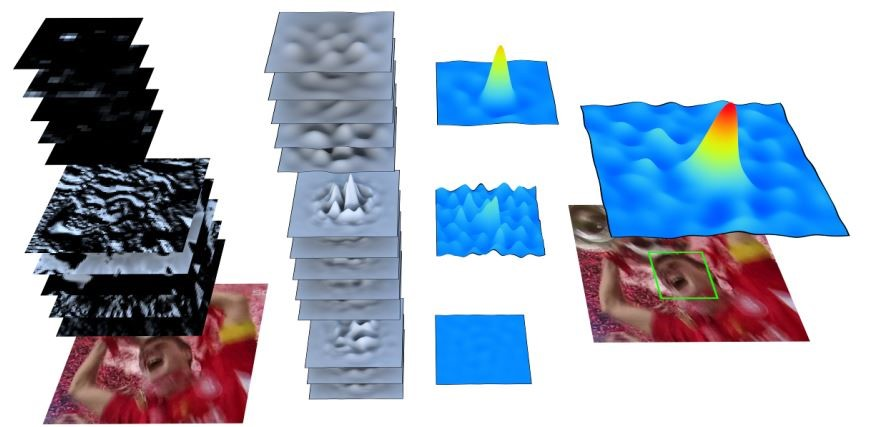
\includegraphics[width=\textwidth]{figures/RW_CCOT.jpg}
    \caption{C-COT的示意图~\cite{C-COT}}
    \label{CCOT_1}
\end{figure}

\begin{table}
    \centering
    \caption{测试用表}
    \wuhao{
    \begin{tabular}{ccc}
    \toprule[1.5pt]
        idx & +(vx,vy)+(w,h) & EAO$\uparrow$ \\ 
        \midrule[1pt]
        T-1 &  & 0.468 \\ 
        T-2 &  & 0.47 \\ 
        中文 &  & 0.471 \\ 
        T-4 &  & 0.472 \\ 
        T-5 &  & 0.479 \\ 
        T-6 & $\surd$ & 0.48 \\ 
        T-7 & $\surd$ & 0.48 \\ 
        \bottomrule[1.5pt]
    \end{tabular}
    }
    \label{CCOT_2}
\end{table}
\clearpage{\pagestyle{empty}\cleardoublepage}
\chapter{总结与展望}

\section{论文总结}
小王将报菜名应用到目标跟踪上来。

甲:“我请你学SiamFC~\cite{SiamFC},SiamRPN~\cite{SiamRPN},SiamMask~\cite{SiamMask}”

乙:“停停”

甲:“我刚说了三算法,你就学不会了?”

乙:“我知道,你就想测试下参考文献。”
\clearpage{\pagestyle{empty}\cleardoublepage}
%%%%%%%%%% 正文部分内容  %%%%%%%%%%

%%%%%%%%%%  参考文献  %%%%%%%%%%
\defaultfont
\bibliographystyle{references/TJUThesis}
\phantomsection
\markboth{参考文献}{参考文献}
\addcontentsline{toc}{chapter}{参考文献}          % 参考文献加入到中文目录
% \nocite{*}                                       % 若将此命令屏蔽掉,则未引用的文献不会出现在文后的参考文献中。
\bibliography{references/reference}

\clearpage{\pagestyle{empty}\cleardoublepage}
% !Mode:: "TeX:UTF-8"

\markboth{发表论文和参加科研情况说明}{发表论文和参加科研情况说明}
\addcontentsline{toc}{chapter}{发表论文和参加科研情况说明}
\chapter*{发表论文和参加科研情况说明}
\setlength{\parindent}{0em}
\textbf{(一)发表的学术论文}
\begin{publist}
\item XXX,XXX. Density and Non-Grid based Subspace Clustering via Kernel Density Estimation[C]. ECML-PKDD 2012, Bristol, UK.(Submitted, Under review)
\item XXX,XXX. A tree parent storage based on hashtable for XML construction[C]. Communication Systems, Networks and Applications, Hongkong, 2010: 325-328. (EI DOI: 10.1109/ICCSNA.2010.5588732)
\end{publist}

\vspace*{1em}
\textbf{(二)申请及已获得的专利(无专利时此项不必列出)}
\begin{publist}
\item XXX,XXX. XXXXXXXXX:中国,1234567.8[P]. 2012-04-25.
\end{publist}
\vspace*{1em}
\textbf{(三)参与的科研项目}
\begin{publist}
\item	XXX,XXX. XX~信息管理与信息系统, ~国家自然科学基金项目.课题编号:XXXX.
\end{publist}
\vfill
\hangafter=1\hangindent=2em\noindent

\setlength{\parindent}{2em}                   % 发表论文和参加科研情况说明
\clearpage{\pagestyle{empty}\cleardoublepage}
\markboth{致\quad 谢}{致\quad 谢}
\addcontentsline{toc}{chapter}{致\qquad 谢} %添加到目录中

\chapter*{致\qquad 谢}

竹板这么一打呀,哎别的咱不夸,

我夸一夸,这个模板先驱——tjuthesis。

这个先驱啊,它究竟好在哪?

它是twtstudio版、jiangqideng版和本版的开路人,就像迎春花。                % 致谢
\clearpage
\end{document}                                 % 结束全文
